% !TeX root = ../main.tex

\chapter{原型实现}
\label{chap:implementation}

\section{系统框架}

\begin{figure}
\centering
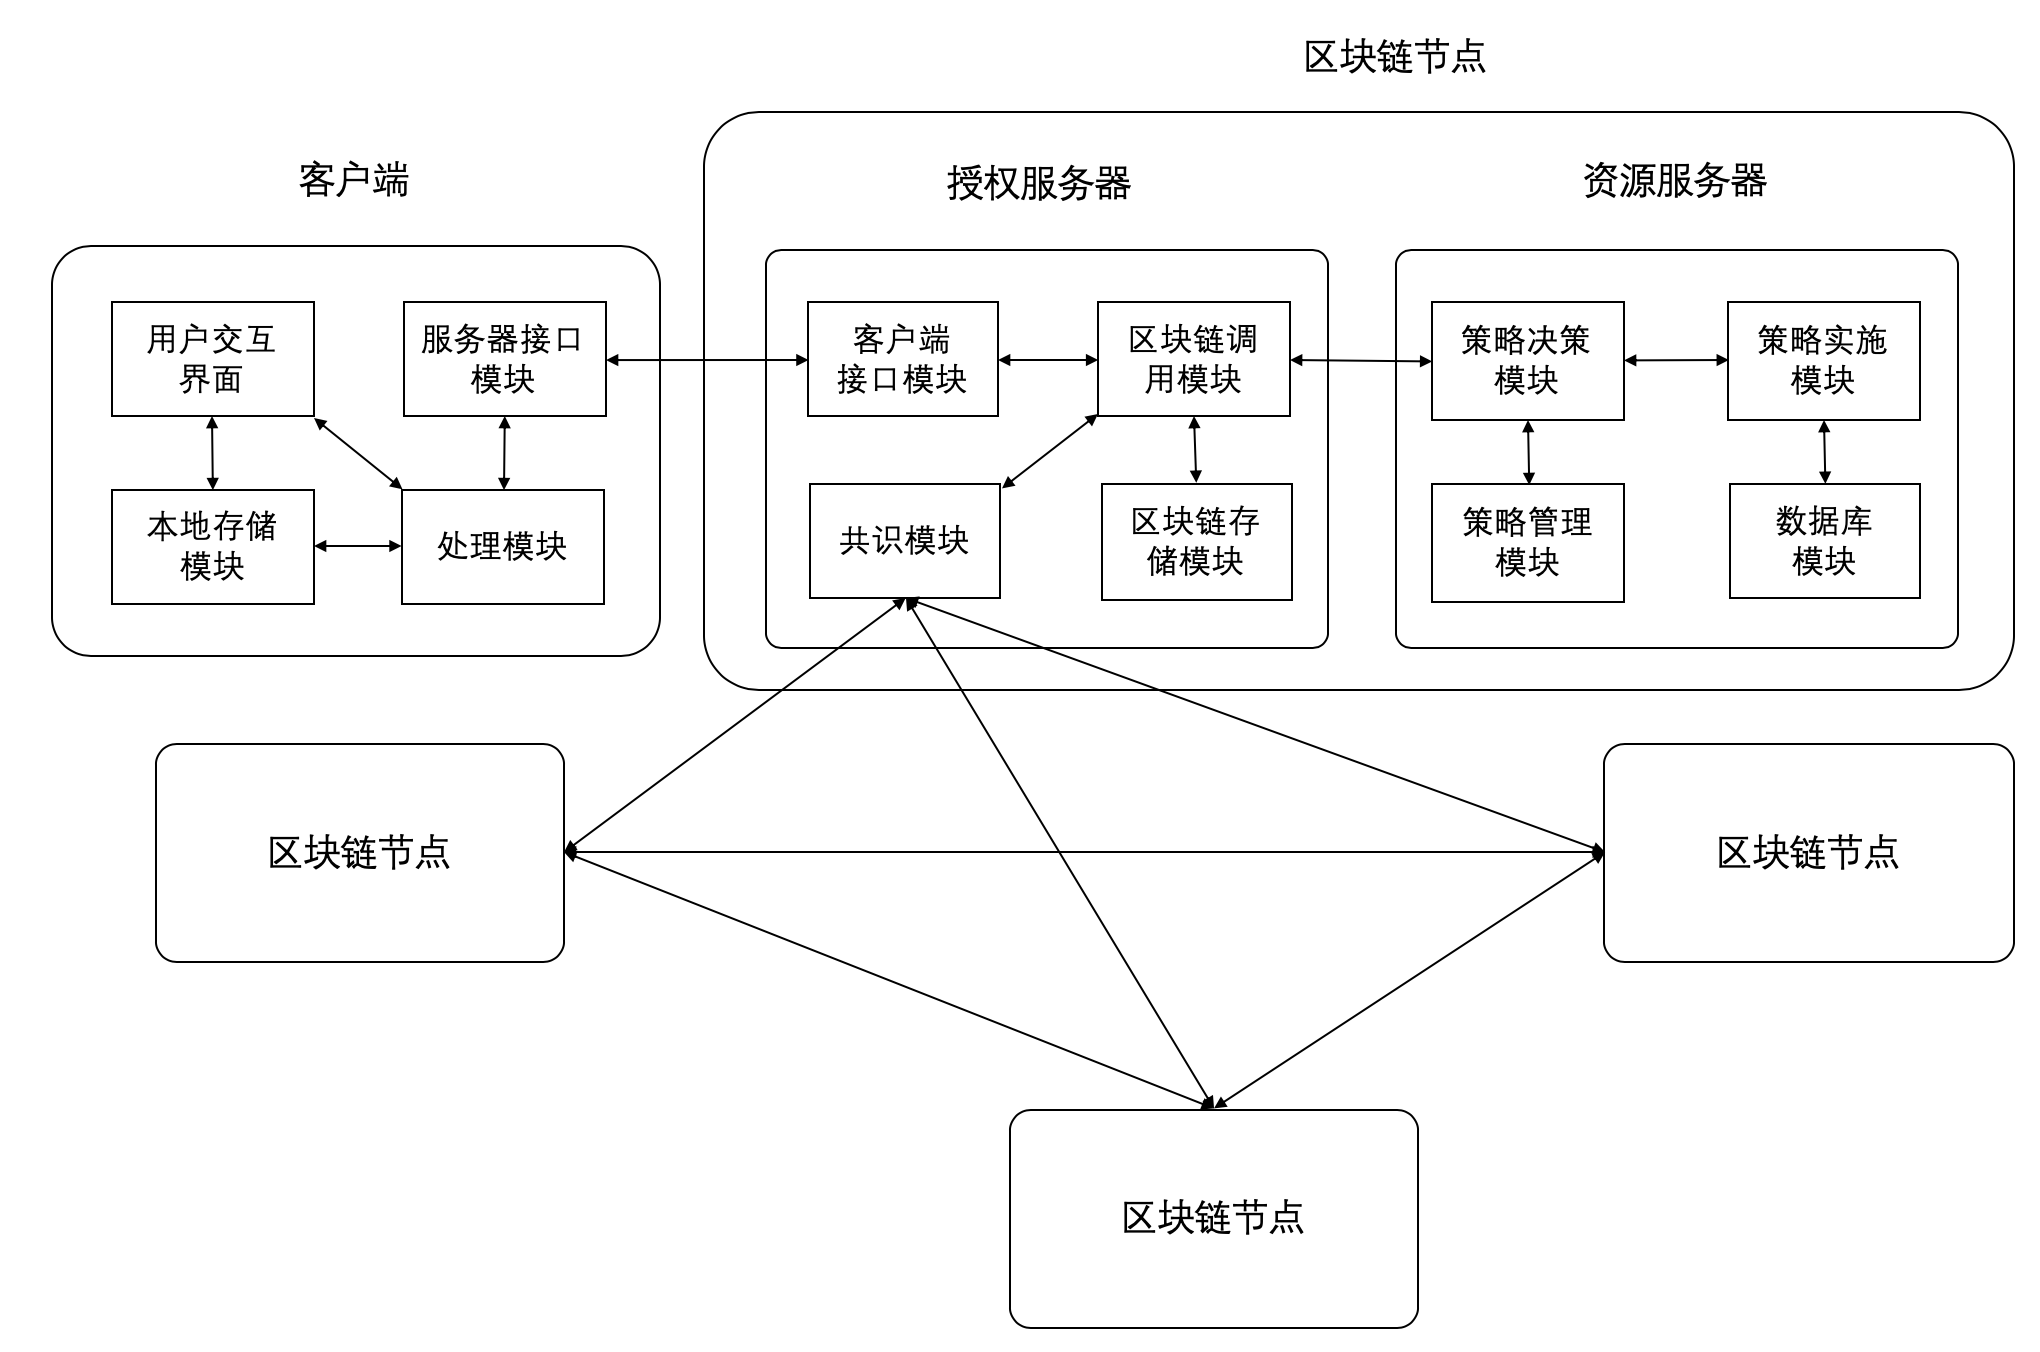
\includegraphics[width=12cm, keepaspectratio]{figures/implementation.png}
\caption{系统实现框架图}
\label{fig:implementation}
\end{figure}

如图\ref{fig:implementation}所示,基于上述协议,我们实现了一个原型系统用于验证设计框架和协议的可行性,并且评估性能和延迟等重要指标。

这一系统采用Go程序语言实现,因为Go语言的并发机制(goroutines和channel通信)帮助构建高性能的网络应用,能提升访问控制系统的性能。为了简化实现,客户端、授权服务器以及资源服务器均采用键值对数据库leveldb存储资源,实际上可以采用现有的各类数据库实现。在区块链网络中,节点间的通信采用HTTP协议实现,未来还可以考虑采用UDP协议提升性能。

\begin{description}
  \item \textbf{客户端}:与框架中“客户端”角色不同,这里实现的客户端用于用户管理自己的账户和密钥,授权其他用户,以及操作可访问的资源。该客户端可以生成并签名授权请求和操作请求,并且和服务器节点进行交互。主要实现以下三个模块:
    \begin{enumerate}
      \item 用户交互界面:用户直接查看和操作的界面,用户可以用来完成账号管理、资源访问、授权等操作。
      \item 本地存储模块:在本地存储用户公私钥对、缓存账号属性等信息。
      \item 处理模块:客户端核心模块,负责数据处理,哈希计算,签名及验证等操作。
      \item 服务器接口模块:与服务器进行通信的模块,封装客户端授权,操作数据发送给服务器,以及解析从服务器收到的回应交给处理模块。
    \end{enumerate}
  \item \textbf{授权服务器}:授权服务器主要实现以下四个模块功能:
    \begin{enumerate}
      \item 客户端接口模块:该模块接受客户端的授权请求和操作请求并转发给核心处理模块,以及将处理结果返回给客户端。
      \item 区块链存储模块:该模块根据核心处理模块的指令,负责区块数据以及状态数据的存储和更新。
      \item 共识模块:该模块发送并接受改进的PBFT协议中的相关消息,包括预准备信息,准备信息,承诺信息,更新视图等。采用多个定时器通过管道实现,保障在限定时间内达成共识产生新区块。
      \item 核心处理模块:该模块处理从客户端或者其他节点接收到的消息,运行前文介绍的区块生成和验证算法。
    \end{enumerate}
  \item \textbf{资源服务器}:资源服务器主要由以下四个模块组成:
    \begin{enumerate}
      \item 策略实施模块:接受用户的操作请求,访问授权服务器中区块链模块获取相应的属性信息,将带属性的操作请求发送给策略决策模块。然后根据返回的决策,决定对数据库模块进行相应操作或者拒绝请求。
      \item 策略决策模块:在接收到来自策略实施模块的带属性的操作请求后,向策略管理模块请求相关的访问控制策略,并根据返回的策略对操作请求进行验证。
      \item 策略管理模块:该模块保存基于属性的访问控制列表,根据策略决策模块的请求返回相应的访问控制策略。
      \item 数据库模块:该模块管理用户存储资源的数据库,并根据策略实施模块的操作请求对数据进行增加、删除、修改以及查询操作。
    \end{enumerate}
\end{description}

\section{客户端实现}

\begin{figure}[htb]
\centering
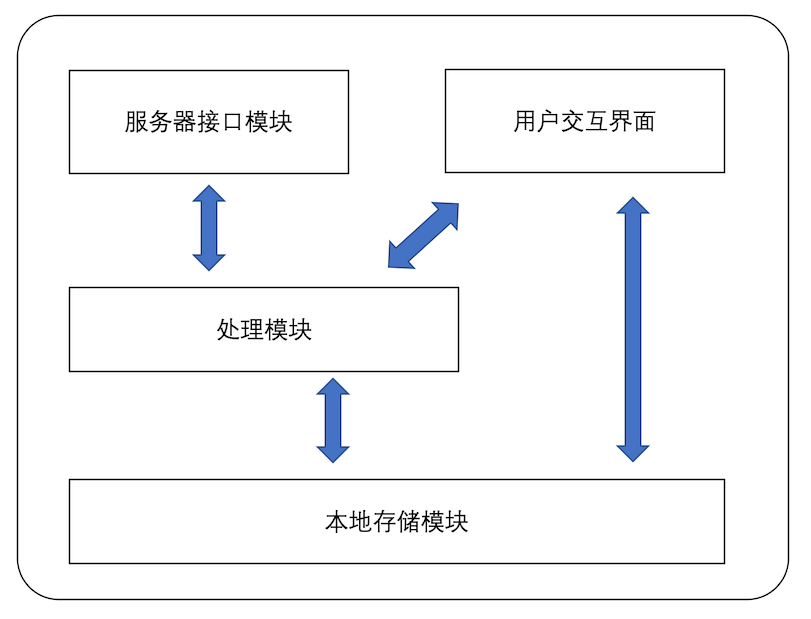
\includegraphics[width=8cm, keepaspectratio]{figures/client.png}
\caption{客户端}
\label{fig:client}
\end{figure}

如图\ref{fig:client}所示,客户端主要包含用户交互界面,本地存储模块,处理模块和服务器接口模块三个部分。其中用户交互界面以网页的形式供用户直接查看和操作,主要由前端代码实现。本地存储模块主要实现用户的账号管理,存储账号的公私钥对,属性等信息。服务器接口模块实现与与服务器通信,根据设计的协议封装用户的操作以及解析从服务器收到的回应数据,并通过调用哈希函数,非对称密码库等密码学组件完成签名及验证等操作。

\subsection{用户交互界面}

\begin{figure}[h]
\centering
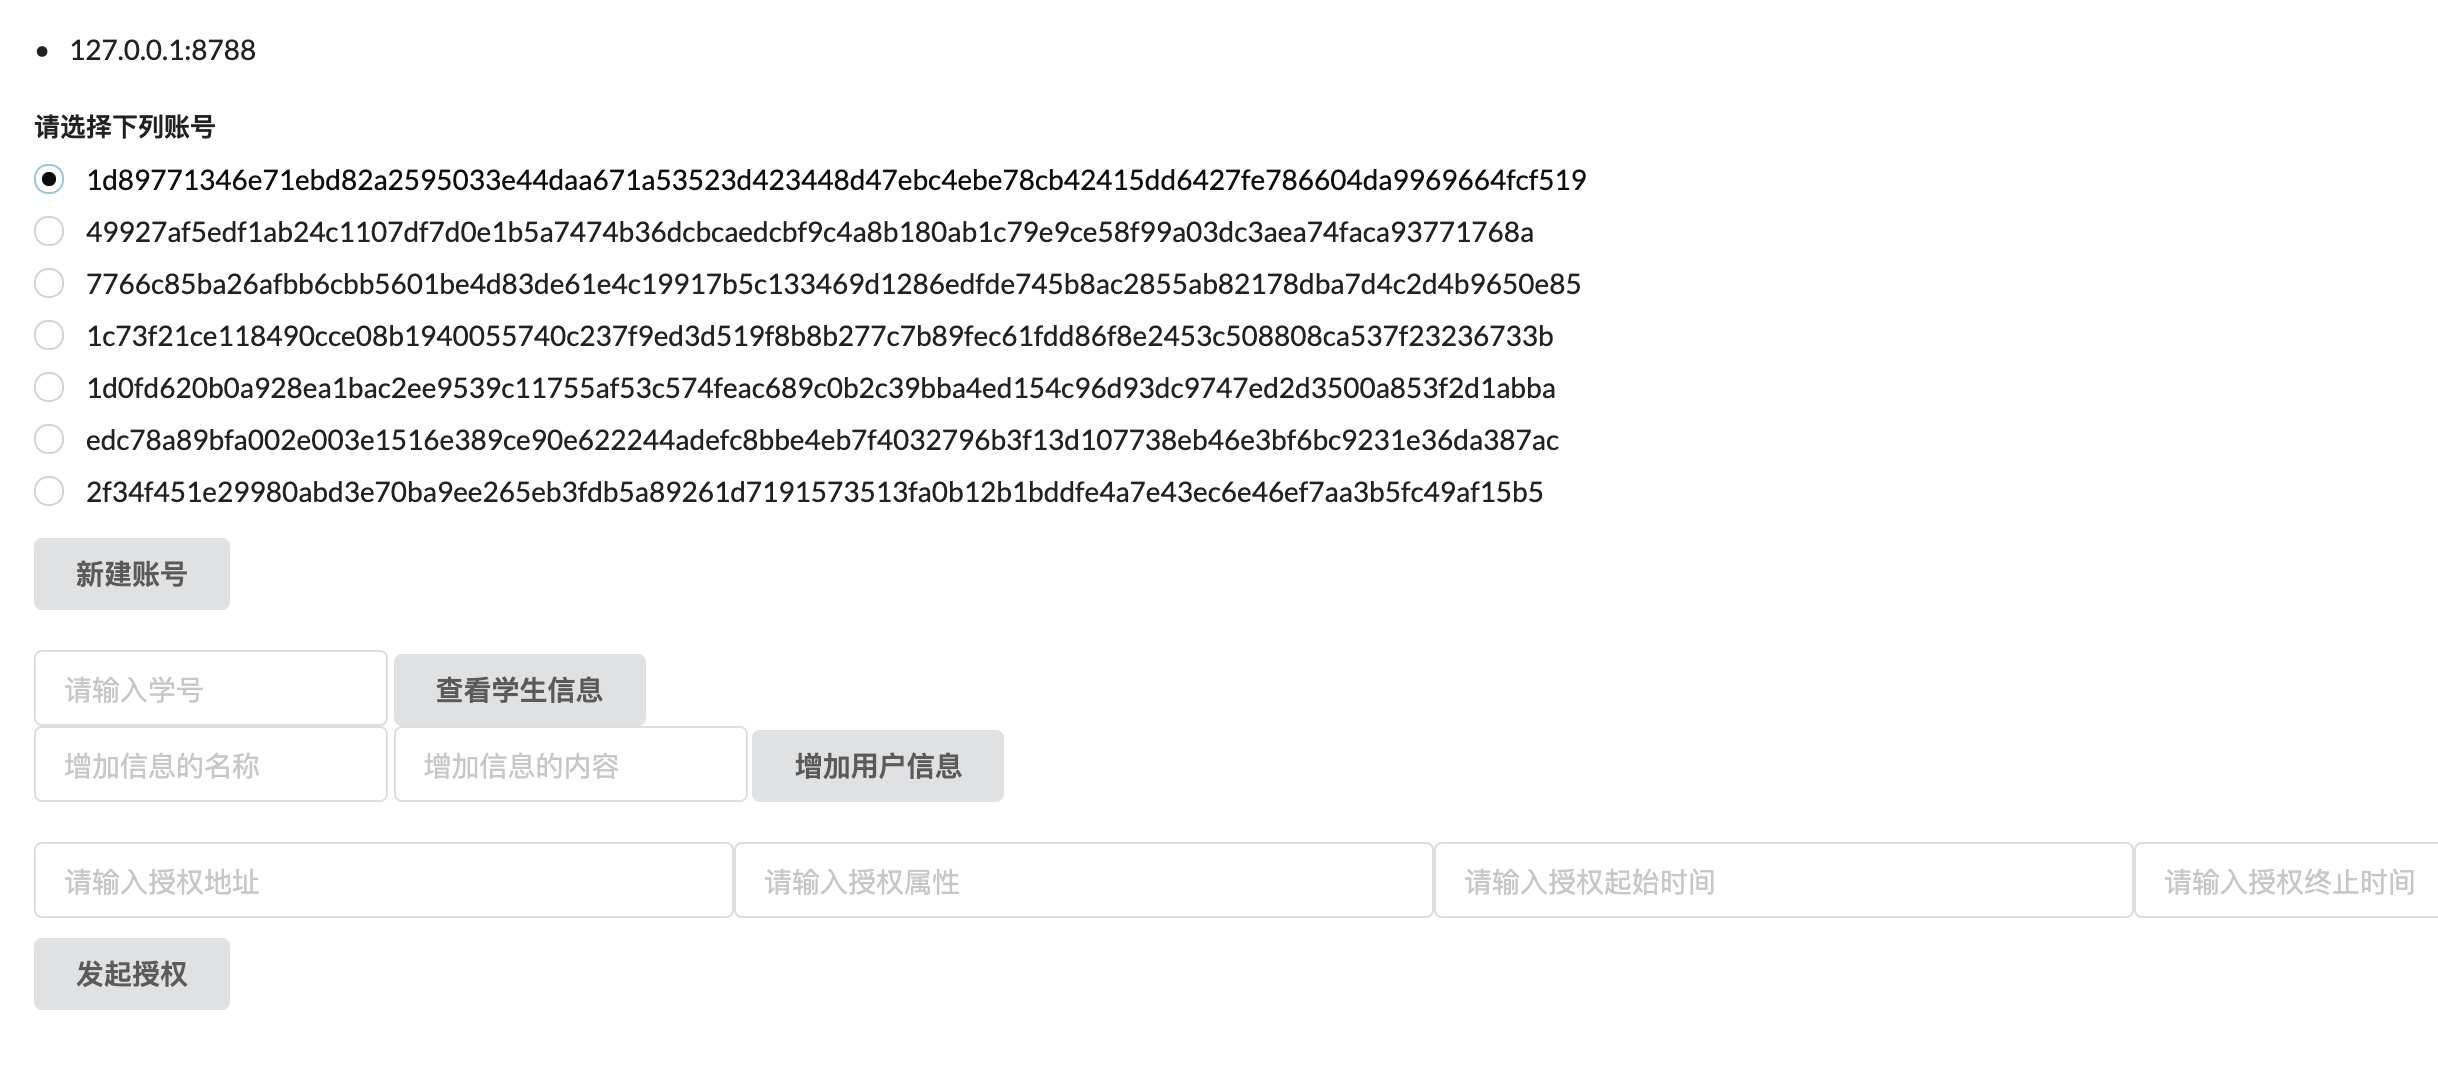
\includegraphics[width=12cm, keepaspectratio]{figures/ui.png}
\caption{用户交互界面}
\label{fig:ui}
\end{figure}

如图\ref{fig:ui}所示,用户交互界面以网页的形式供用户直接查看和操作,用户可以通过“新建账号”按钮创建账号,并选择当前本地已有的任意账号。选定账号后,用户可以通过查看信息,增加信息,修改信息,删除信息等接口对资源进行操作。并且可以通过授权接口,将自己的属性在选定的时间内授权给其他账号。交互界面中,html代码实现界面各元素,css代码实现各文本框及按钮等元素的样式,js代码实现各按钮的交互功能,以及和处理模块进行数据交互。

\subsection{处理模块}

处理模块负责客户端的数据处理,一方面接受来自用户交互界面的账户操作,根据请求数据对本地存储模块进行更新。另一方面,处理用户发起的授权操作和资源操作请求,将请求数据转发到服务器接口模块,由该模块解析并重新封装后发送给服务器。数据处理的过程中调用哈希函数,椭圆曲线等密码学库完成哈希计算,消息签名及签名验证等操作。

\subsection{本地存储模块}

本地存储模块存储用户公私钥对信息,当处理模块需要时提供用于签名或验证。现有各类区块链钱包管理系统用于安全管理账户信息,为了实现简单,本系统以json格式的文件对账户信息进行存储。

\subsection{服务器接口模块}

服务器接口模块负责与服务器进行通信。封装客户端授权数据和操作数据发送给服务器,以及解析从服务器收到的回应转发给处理模块。

\section{授权服务器实现}

\begin{figure}[htb]
\centering
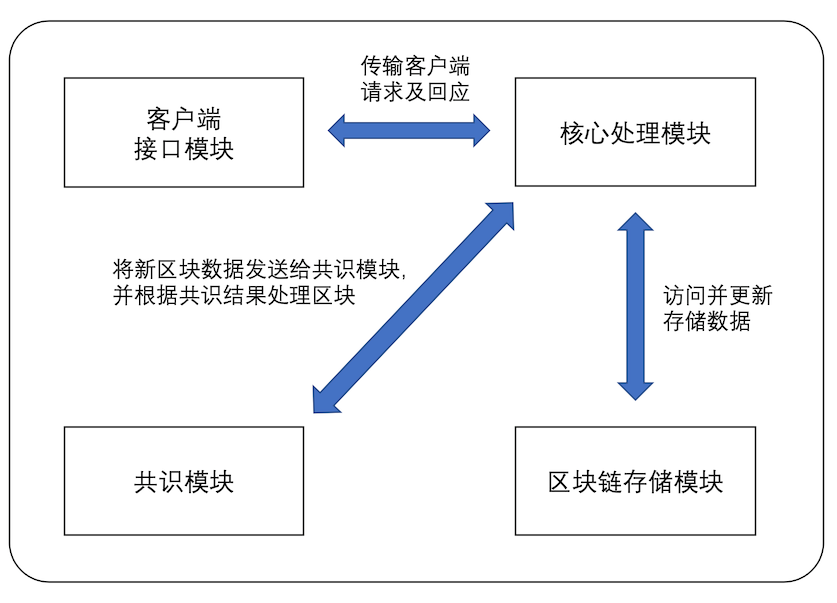
\includegraphics[width=8cm, keepaspectratio]{figures/imple-auth.png}
\caption{授权服务器实现框架}
\label{fig:imple-auth}
\end{figure}

授权服务器主要实现客户端接口模块,区块链调用模块,区块链存储模块以及共识模块四个模块功能。其中客户端接口模块负责接受客户端的授权请求和操作请求并转发给核心处理模块,以及将处理结果返回给客户端。区块链存储模块根据核心处理模块的指令,负责区块数据以及状态数据的存储和更新。共识模块与其他区块链节点相连,发送并接收共识协议中的相关消息,包括预准备信息,准备信息,承诺信息,更新视图等。采用多个定时器通过管道实现,保障在限定时间内达成共识产生新区块。核心处理模块负责处理从客户端或者其他区块链节点接收到的数据,运行第\ref{sec:b-oauth}介绍的授权验证、区块生成等算法。

\subsection{客户端接口模块}

该模块接受客户端的授权请求和操作请求并转发给处理器模块,以及将处理结果返回给客户端。根据预先定义的授权和操作数据结构,负责数据的解析和封装。

\subsection{核心处理模块}

该模块处理从客户端或者其他节点接收到的消息,将通过验证的授权数据存放在授权池,根据共识模块的信号从授权池中选取授权打包成新区块,提交给共识模块。

\subsection{区块链存储模块}

该模块负责存储区块链数据,采用leveldb数据库对区块链链上数据进行存储。该模块在每次核心处理模块启动时,需要提供达成共识的区块链历史数据。在共识模块达成共识后,由核心处理模块将新区块数据发送给存储模块写入数据库。

\subsection{共识模块}

\begin{figure}[ht]
  \centering%
  \subcaptionbox{“预准备消息”数据结构\label{fig:pre-prepare}}
    {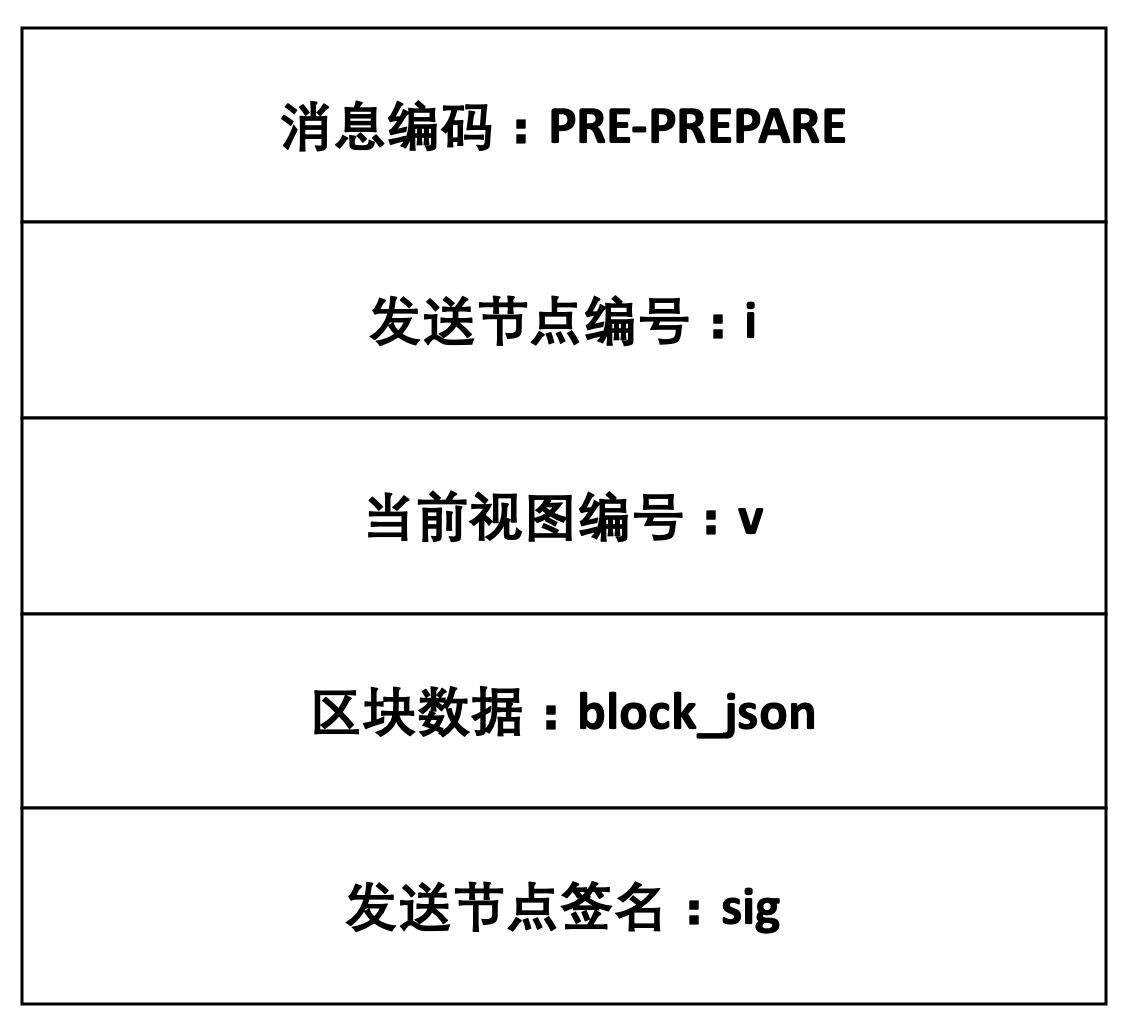
\includegraphics[width=6cm]{figures/pre-prepare.png}}%
  \hspace{2em}%
  \subcaptionbox{“准备消息”数据结构\label{fig:prepare}}
      {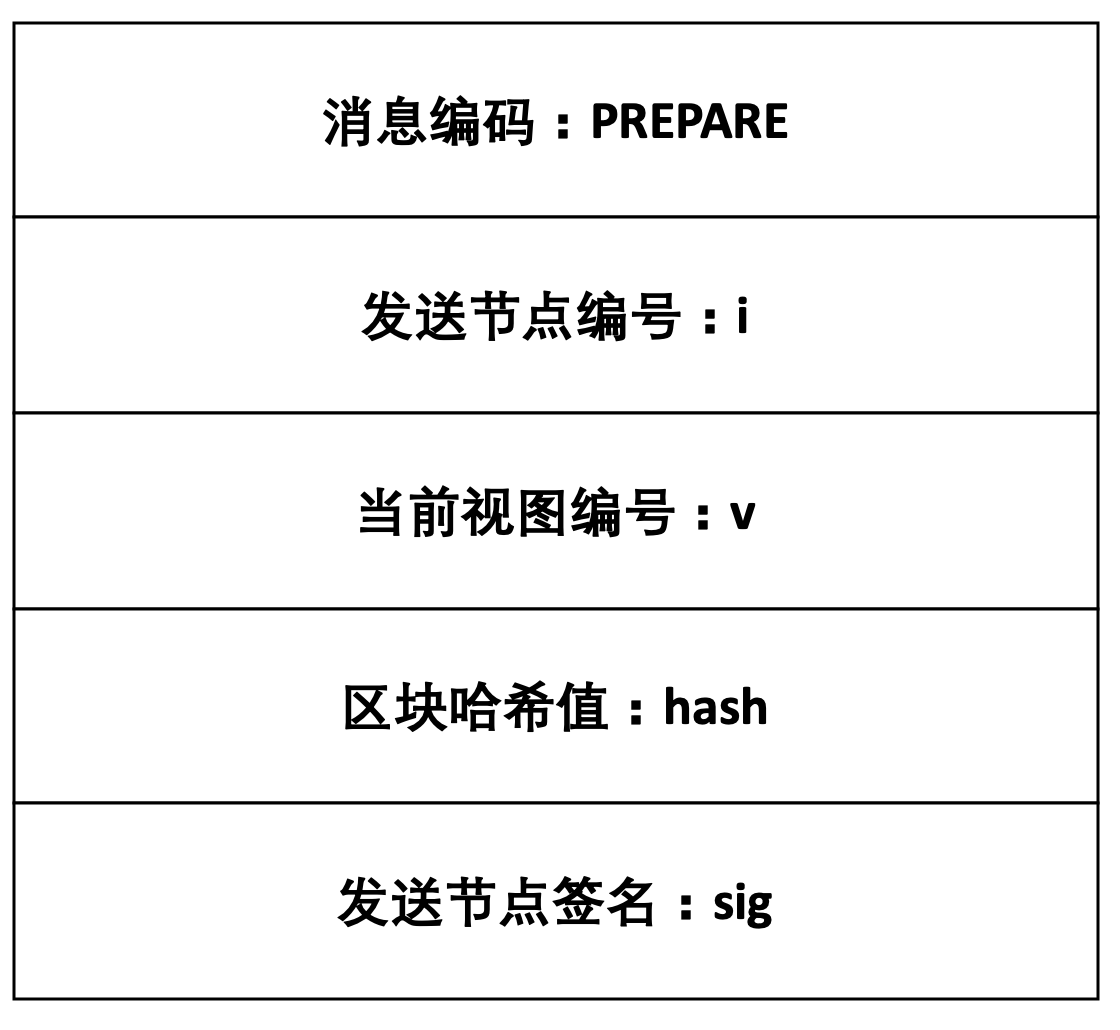
\includegraphics[width=6cm]{figures/prepare.png}}

  \subcaptionbox{“承诺消息”数据结构\label{fig:commit}}
      {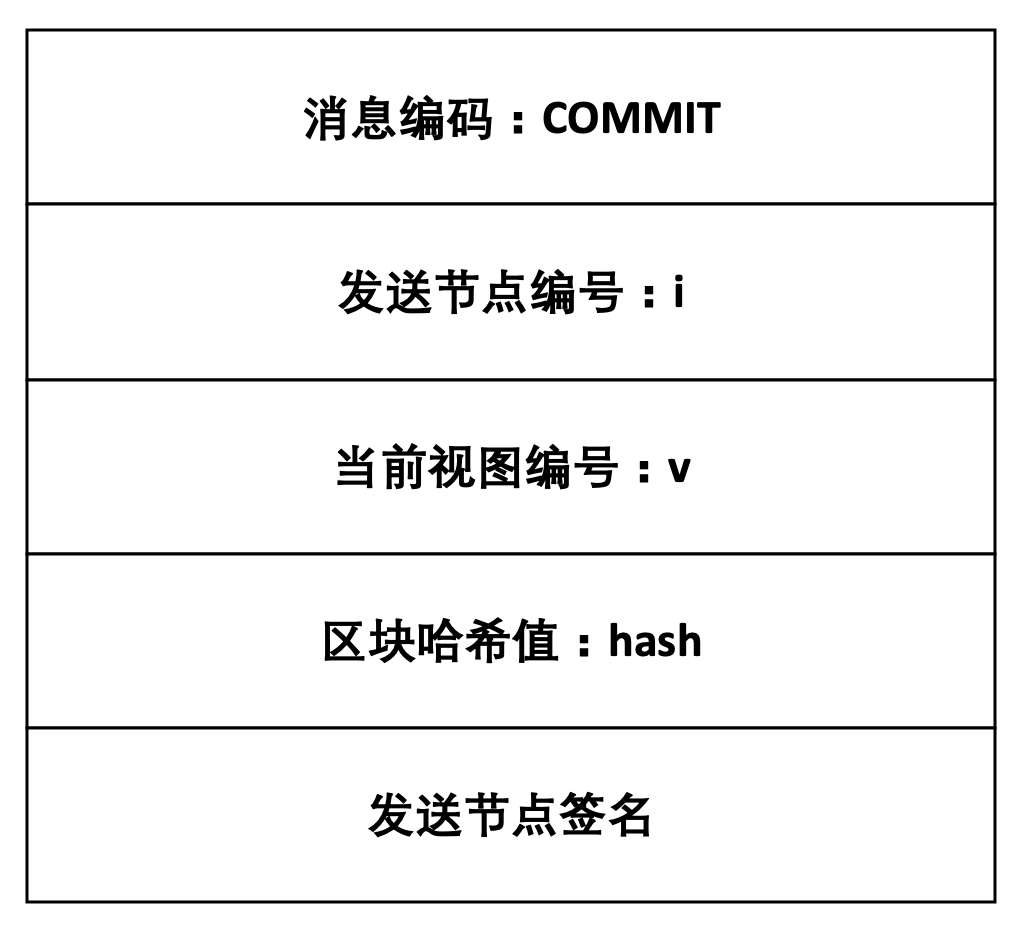
\includegraphics[width=6cm]{figures/commit.png}}
  \hspace{2em}%
  \subcaptionbox{“视图更新消息”数据结构\label{fig:viewchange}}
      {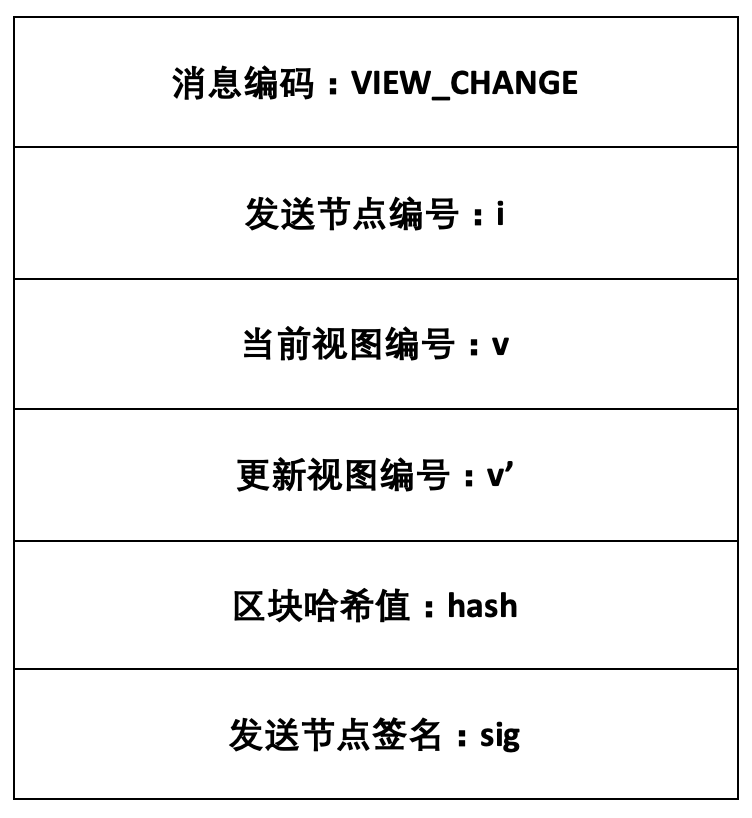
\includegraphics[width=6cm]{figures/viewchange.png}}
  \caption{共识协议中各类消息的数据结构}
  \label{fig:pbft-data}
\end{figure}

共识模块中首先设计了各类消息的数据结构,如图\ref{fig:pbft-data}所示。各节点的共识模块之间通过http协议进行通信,并按照规定的数据结构对消息进行封装。

\begin{figure}
\centering
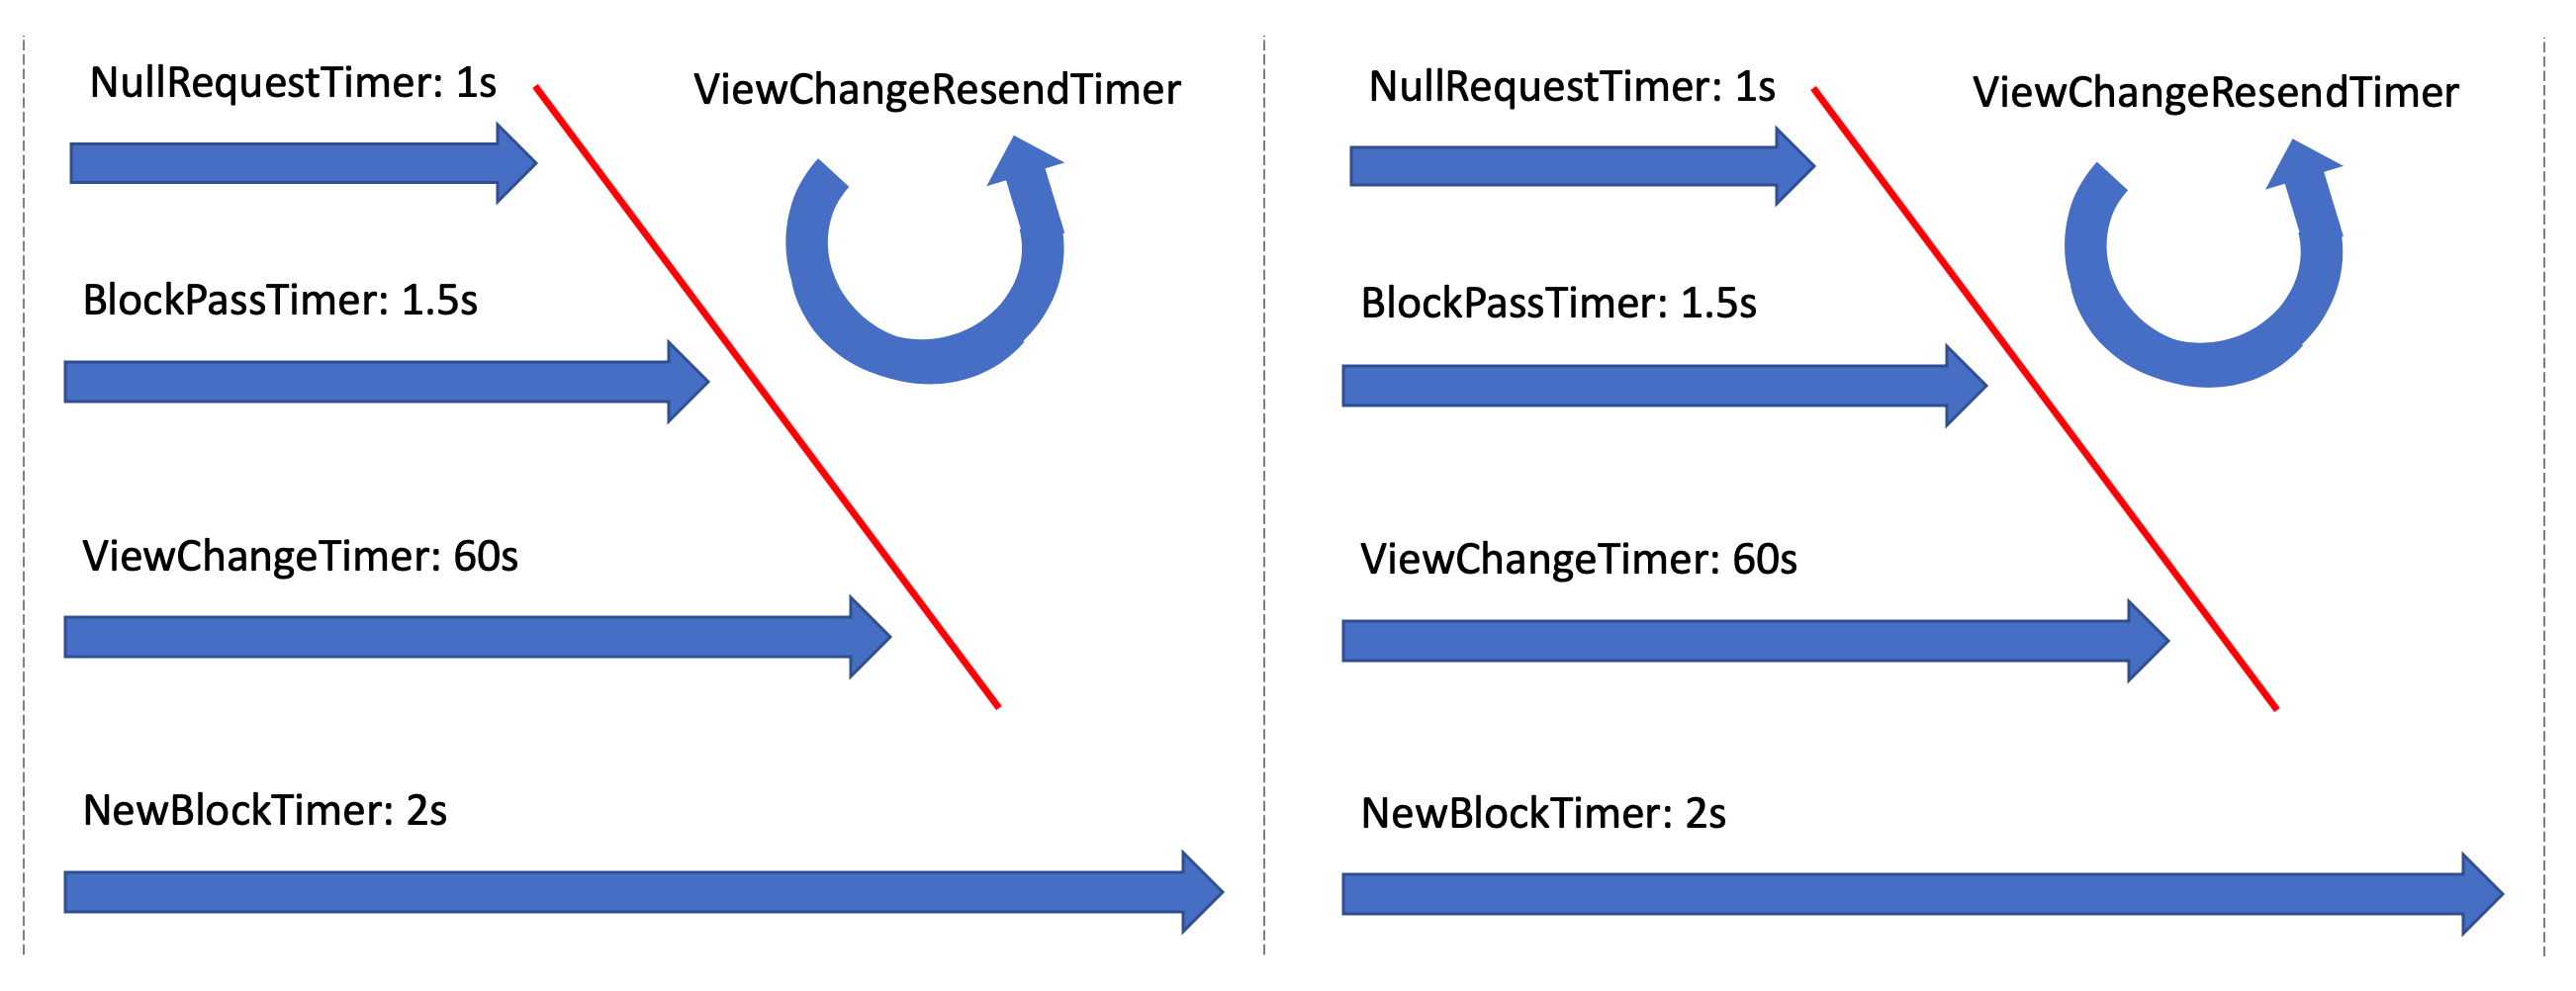
\includegraphics[width=12cm, keepaspectratio]{figures/timer.png}
\caption{定时器工作流程}
\label{fig:timer}
\end{figure}

该模块采用第\ref{subsec:adapted-pbft}节中介绍的共识协议,主要通过若干定时器启动函数,保障协议的正常进行。如图\ref{fig:timer},该系统中,正常情况下由NewBlockTimer每2秒启动一次NewBlock函数,开始一轮新的共识。当每轮共识开始时,启动NullRequestTimer和BlockPassTimer,如果节点在1秒内没有接收到来自主节点的消息,则NullRequestTimer到期。如果节点在1.5秒内没有收到足够多的“承诺消息”表示共识达成,则BlockPassTimer到期。为了保障在一定时间后主节点切换,ViewChangeTimer设置为每60秒到期一次,无法中断。这三个定时器到期,节点都会发起视图切换,开始不断循环ViewChangeResendTimer尝试切换到下一个视图,直到与其他节点达成共识成功切换视图为止。

\section{资源服务器实现}

\begin{figure}[ht]
\centering
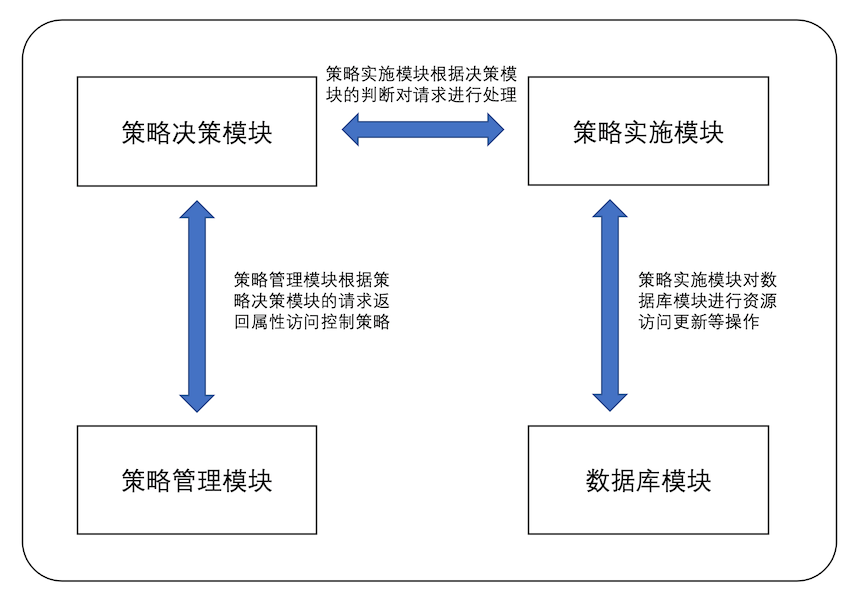
\includegraphics[width=8cm, keepaspectratio]{figures/imple-resource.png}
\caption{资源服务器实现框架}
\label{fig:imple-resource}
\end{figure}

如图\ref{fig:imple-resource}所示,资源服务器主要由以下四个模块组成,数据库模块管理用户存储资源的数据库,并根据访问控制模块的验证结果对数据进行操作。策略管理模块保存基于属性的访问控制列表。策略决策模块对访问请求进行决策。策略实施模块根据策略决策模块的判断对数据库模块进行操作,并回应请求。

\subsection{策略实施模块}

策略实施模块接收来自用户的操作请求,如果消息与签名不符合则直接拒绝该请求。在验证签名后,策略实施模块根据当前时间补充上时间戳字段作为环境属性,提交给策略决策模块。等待策略决策模块回应决策结果后,策略实施模块将操作请求中具体操作的信息发送给数据库模块。最后将数据库模块返回的操作结果发送给请求用户。

\subsection{策略决策模块}

策略决策模块接收来自策略实施模块的带属性的操作请求,解析出其中主体属性、客体属性、操作属性以及环境属性,根据各属性从策略管理模块中获取相关的访问控制策略。控制策略列表中的各策略包含主体属性、客体属性、操作属性以及环境属性四个部分,其中主体属性、客体属性以及操作属性由逻辑表达式构成,当操作请求中的各项属性满足逻辑表达式即满足。环境属性只包含时间戳,由起始时间和终止时间两个字段组成,当操作请求中的时间戳在起始时间和终止时间组成的区间内即满足。如果操作请求满足访问控制策略列表中任何一项策略,则通过验证。策略决策模块将验证后的结果返回给策略实施模块。

\subsection{策略管理模块}

本原型系统不考虑策略列表的初始化和更新,策略管理模块只负责存储访问控制策略列表,当接受到策略决策模块关于带有某些属性的访问策略请求时,返回对应策略。为了简化实现,访问控制列表以json形式文件存储。

\subsection{数据库模块}

该原型实现中,数据库模块采用LevelDB键值数据库存放管理用户信息,每个用户拥有唯一编号。可以根据该编号查询用户信息,以及对信息进行增加、删除、修改等操作。操作请求的数据结构主要包含用户编号、操作类型、操作字段、操作值四个数据。其中当操作类型为查询时,操作字段和操作值可以为空。当操作类型为删除时,操作值可以为空。当操作类型为新增和修改时,所有字段都不能为空。

\section{性能测试}

\begin{figure}
\centering
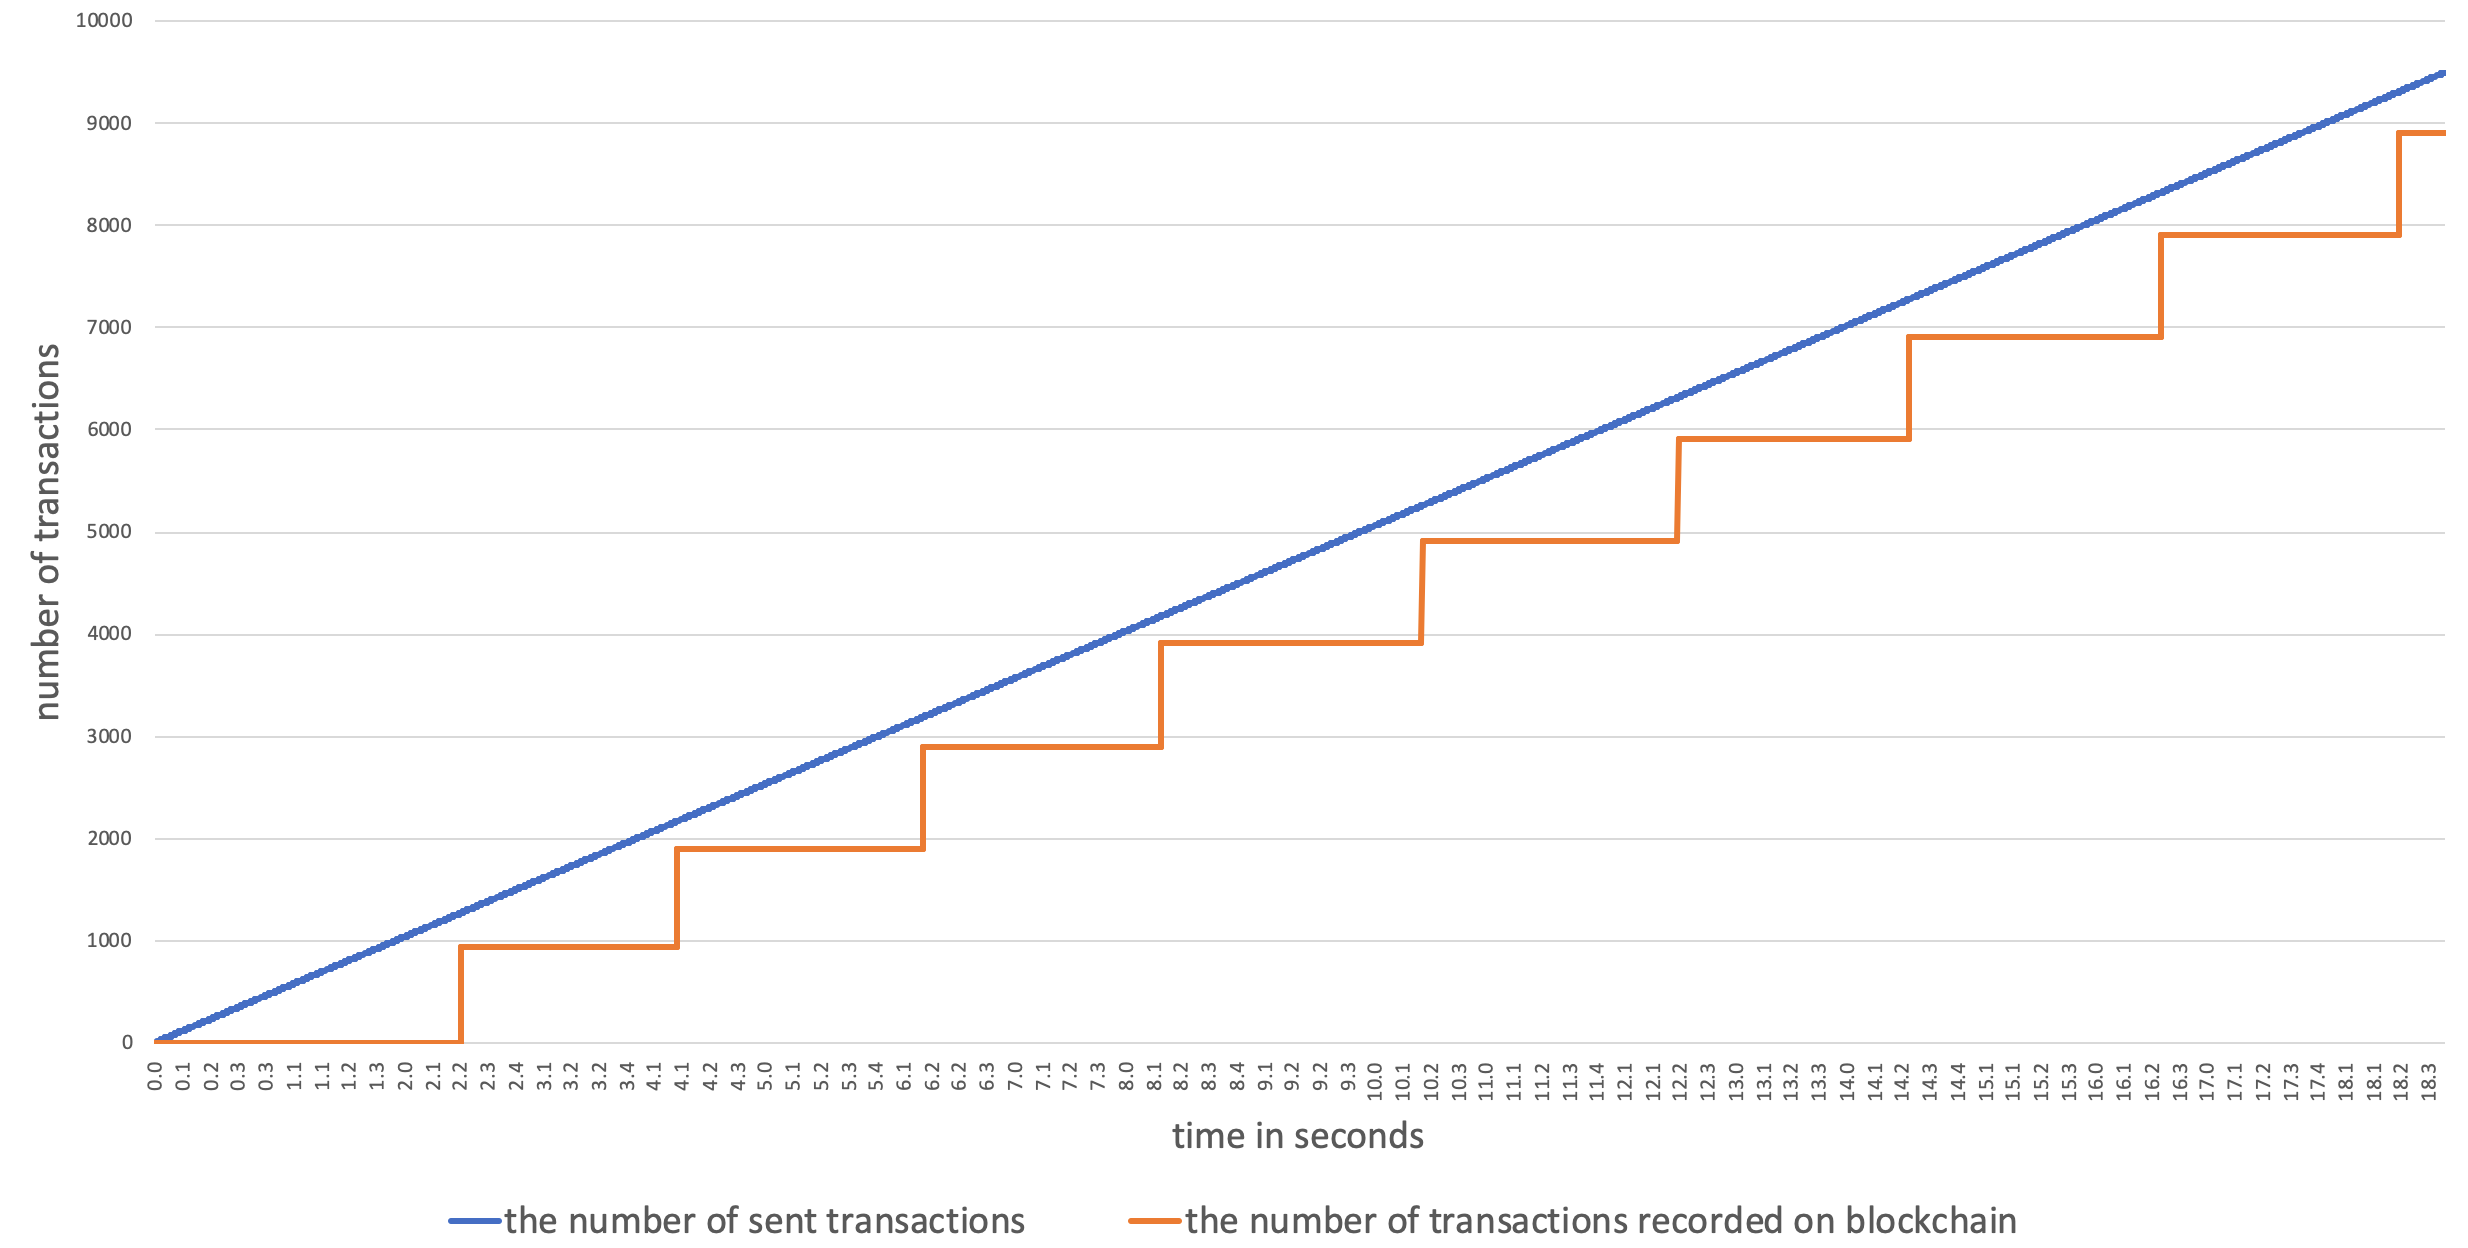
\includegraphics[width=12cm, keepaspectratio]{figures/performance.png}
\caption{性能测试}
\label{fig:performance}
\end{figure}

我们在微软云平台上部署了四个区块链节点,每个节点采用标准的D2s v3型号服务器,拥有2 vCPU,2G内存以及1000 MBps网络带宽。为了测试系统性能,我们生成了1000对公私钥对来模拟1000个用户,每个用户拥有不同的属性,还在随机用户之间生成了10000个随机的授权操作,用于模拟现实中的授权行为。

测试授权数据以每秒500个授权的速率发送给4个节点,区块链网络在大概21秒的时间里成功处理了这些请求。发送的分布时间如图\ref{fig:performance}所示。该网络每2秒生成一个新区块,并且每个区块最多包含1000个授权请求(这一限制设置在代码中)。每个区块包含的授权信息数量如图\ref{fig:performance}所示。实验证明了该系统可以达到每秒处理500个授权请求并且平均延迟在1秒左右,这说明该框架和协议可以应用于部分现实场景中。并且在性能上还可以通过增加服务器性能、带宽,优化通信协议等方式提升。